\documentclass[11pt]{article}
\usepackage{amsmath,amssymb,amsthm}
\usepackage{geometry}
\usepackage{booktabs}
\usepackage{hyperref}
\usepackage{natbib}
\usepackage{tikz}
\usetikzlibrary{arrows.meta,positioning}
\usepackage{graphicx}
\geometry{margin=1in}

\newcommand{\psii}{\psi}
\newcommand{\iotaop}{\iota}
\newcommand{\gammaop}{\gamma}
\newcommand{\rav}{\mathrm{rav}}
\newcommand{\vecx}{\vec{x}}
\newcommand{\vecz}{\vec{z}}

\theoremstyle{definition}
\newtheorem{definition}{Definition}
\newtheorem{lemma}{Lemma}

\title{The Transformer Block at the Theoretical Minimum:\\
Memory-Optimal Normalization and Feed-Forward Layers via the\\
Mathematics of Arrays}
\author{Lenore M. Mullin \and Ga\'etan Hains}
\date{Draft v0.1 --- \today}

\begin{document}
\maketitle

\begin{abstract}
This paper extends the Mathematics of Arrays (MoA) treatment of scaled
dot-product attention developed in our companion papers on the forward
pass (arXiv:2606.07713), the backward pass (HAL-05659212), and
memory-optimal inference, to the two remaining components of a standard
transformer block: the normalization layer (RMSNorm, with LayerNorm as a
specialization) and the position-wise feed-forward network (a gated MLP
in the SwiGLU family). We derive Denotational Normal Form (DNF)
expressions for the forward, backward, and fused forward+backward passes
of both components, establish memory-optimal cost functions in the same
style as the attention papers ($M_{\text{fwd}}$, $M_{\text{bwd}}$,
$M_{\text{fwd+bwd}}$), and show that the intermediate arrays materialized
by naive implementations --- the normalization statistic, the
un-gated activation, and the gate pre-activation --- can be eliminated
by substitution under MoA's outer-product compatibility conditions,
exactly as $A$ and $O$ were eliminated in the fused attention kernel.
Combined with the prior three papers, this gives a complete
memory-optimal account of a single transformer block: normalization,
attention, normalization, and feed-forward. Verification follows the
established methodology: Fortran~90 and C/OpenMP reference
implementations checked against PyTorch forward and autograd values.
\end{abstract}

\section{Introduction and Positioning}

Papers I and II of this series established memory-optimal DNF/ONF
formulations for the forward, backward, and fused passes of scaled
dot-product attention, with cost functions
\[
M_{\text{bwd}} = n^2 + 4nd_k + 3nd_v, \qquad
M_{\text{fwd+bwd}} = 4nd_k + 4nd_v
\]
and a companion inference paper derived four artifacts (decode DNF,
C/OpenACC GPU kernel, KV-cache, GQA/MQA) verified against PyTorch SDPA.
Attention is, however, only one of the two sublayers in a transformer
block; the other is normalization (applied twice, pre- or post-sublayer)
and the position-wise feed-forward network. A memory-optimal account of
attention alone cannot support end-to-end claims about a transformer
layer's memory traffic --- normalization and the FFN together account
for a majority of a layer's parameters and, for long sequences, a
non-trivial share of its activation memory. This paper closes that gap.

We deliberately hold two related topics out of scope, to be treated as
separate future papers: (1) dynamic KV-cache management and speculative
decoding, which extend the \emph{inference} paper rather than this one;
and (2) Mixture-of-Experts routing, which requires MoA's primitives to
handle data-dependent, irregular dispatch and is a research question in
its own right rather than a direct extension of the dense-array
machinery used here.

\section{Notation}

We retain the conventions established in Papers I--III without change:
$\rho$ denotes shape, the five MoA primitives are $\psii$ (psi
indexing, written infix as $\langle i \rangle \psii A$), $\iotaop$
(index generator), $\rho$ (shape), $\gammaop$ (the DNF$\to$ONF
translator), and $\rav$ (ravel/flatten); MoA multiplication is written
$\times$; batch index $b$ is always explicit; scalars carry full
three-index subscripts; vectors carry arrow notation; there is no
row/column vector language; gradient arrays are named ($G_X$, $G_\gamma$,
\ldots) rather than written with partial-derivative notation.

New symbols introduced in this paper:
\begin{itemize}
  \item $X \in \mathbb{R}^{B\times N\times D}$: block input, batch $b$,
  sequence position $n$, model dimension $d$.
  \item $\vec{\gamma} \in \mathbb{R}^D$: learned RMSNorm scale (LayerNorm
  additionally has a learned bias $\vec\beta$).
  \item $r_{b,n} \in \mathbb{R}$: the per-token RMSNorm statistic
  (scalar, hence full subscripting, no arrow).
  \item $Z \in \mathbb{R}^{B\times N\times D}$: normalized output.
  \item $W_{\mathrm{gate}}, W_{\mathrm{up}} \in \mathbb{R}^{D\times
  D_{\mathrm{ff}}}$, $W_{\mathrm{down}} \in \mathbb{R}^{D_{\mathrm{ff}}
  \times D}$: FFN weights.
  \item $U, V, H \in \mathbb{R}^{B\times N \times D_{\mathrm{ff}}}$:
  gate pre-activation, up-projection, and gated hidden state.
  \item $F \in \mathbb{R}^{B\times N\times D}$: FFN output.
\end{itemize}

\section{RMSNorm: Forward DNF}

For fixed $b,n$, write $\vecx = \langle b,n\rangle \psii X \in
\mathbb{R}^D$. The RMSNorm statistic is a reduction over the innermost
axis:
\[
r_{b,n} = \sqrt{\frac{1}{D}\sum_{d=1}^{D} x_{b,n,d}^2 + \epsilon}.
\]
The DNF for the output at index $(b,n,d)$ is
\[
z_{b,n,d} = \gamma_d \cdot \frac{x_{b,n,d}}{r_{b,n}}.
\]
As in the softmax case treated in Paper I, this is a two-pass DNF: a
reduction pass producing the shape-$(B,N)$ array $r$, followed by an
elementwise pass combining $r$, $X$, and $\vec\gamma$ under MoA's
outer-product compatibility (the same compatibility condition used to
eliminate materialized intermediates in the fused attention kernel).
Under $\gammaop$-translation to ONF, the reduction pass tiles over $D$
with a running sum-of-squares accumulator, and the elementwise pass
fuses directly onto the reduction's output without materializing an
intermediate $\hat X = X/r$ array --- $\hat x_{b,n,d}$ is recomputed
on-the-fly inside the elementwise pass, exactly as $A$ is recomputed
on-the-fly in fused attention.

\paragraph{LayerNorm as a specialization.} LayerNorm replaces $r_{b,n}$
with the standard deviation about the mean and adds a learned bias
$\vec\beta$:
\[
\mu_{b,n} = \frac{1}{D}\sum_d x_{b,n,d}, \qquad
\sigma_{b,n} = \sqrt{\frac{1}{D}\sum_d (x_{b,n,d}-\mu_{b,n})^2 + \epsilon},
\qquad
z_{b,n,d} = \gamma_d\frac{x_{b,n,d}-\mu_{b,n}}{\sigma_{b,n}} + \beta_d.
\]
This costs one additional reduction pass (the mean) relative to
RMSNorm; the DNF/ONF and fusion argument are otherwise identical. We
carry RMSNorm as the primary case in what follows since it is the
dominant choice in current large-scale models, and note LayerNorm
results by the same substitution wherever they differ materially.

\section{RMSNorm: Backward DNF}

Given upstream gradient $G_Z$ (same shape as $Z$), we require $G_X$ and
$G_{\vec\gamma}$. Write $\hat x_{b,n,d} = x_{b,n,d}/r_{b,n}$ (recomputed,
never materialized, as above).

\begin{lemma}[RMSNorm input gradient]
\[
G_{X,b,n,e} = \frac{1}{r_{b,n}}\left[
G_{Z,b,n,e}\,\gamma_e \;-\; \frac{\hat x_{b,n,e}}{D}
\sum_{d=1}^{D} G_{Z,b,n,d}\,\gamma_d\,\hat x_{b,n,d}
\right].
\]
\end{lemma}

\begin{proof}[Derivation sketch]
$z_{b,n,d} = \gamma_d x_{b,n,d} r_{b,n}^{-1}$. Differentiating $r_{b,n}$
with respect to $x_{b,n,e}$ gives $\partial r_{b,n}/\partial x_{b,n,e} =
x_{b,n,e}/(D\, r_{b,n})$, hence
\[
\frac{\partial z_{b,n,d}}{\partial x_{b,n,e}} =
\gamma_d\, r_{b,n}^{-1}\Big(\delta_{de} - \hat x_{b,n,d}\hat
x_{b,n,e}/D\Big).
\]
Contracting with $G_{Z,b,n,d}$ over $d$ and collecting terms gives the
stated form. Note the structural parallel to the softmax-VJP row-sum
correction in the backward attention paper: both gradients are a
``local'' term minus a mean-subtracted correction term, and both
corrections are reductions that can be fused into a single accumulator
pass rather than materialized separately.
\end{proof}

\begin{lemma}[RMSNorm scale gradient]
\[
G_{\gamma,d} = \sum_{b,n} G_{Z,b,n,d}\,\hat x_{b,n,d}.
\]
\end{lemma}

This is a reduction over both batch and sequence axes and, in ONF, tiles
independently of the $G_X$ pass, so the two gradients can be computed in
a single fused traversal of $X$, $G_Z$, and $r$ without a second
materialization of $\hat X$.

\section{RMSNorm: Fused Forward+Backward Cost}

Following the accounting convention of Paper II ($M$ = number of
$D$-sized (or $D\times$batch$\times$seq-sized) reads/writes of
activation memory, weights excluded), the naive implementation
materializes $X$, $r$, $\hat X$, $Z$, then in the backward pass re-reads
$X$, $r$, $G_Z$ and writes $G_X$, $G_\gamma$ --- six full arrays.
Because $\hat X$ is eliminated by recomputation in both passes (Section
3--4), and $r$ is a $(B,N)$-shaped array that is $D\times$ cheaper than
a full activation array, the fused cost is
\[
M^{\mathrm{norm}}_{\text{fwd+bwd}} = 4nd \quad \text{(per batch element, } n
\text{ sequence positions, } d = D\text{)},
\]
counting $X$, $Z$, $G_Z$, $G_X$ as the only full-size arrays touched,
with $r$ and $G_\gamma$ contributing lower-order $O(n)$ and $O(d)$
terms respectively. This is the norm-layer analogue of the attention
fused cost $M_{\text{fwd+bwd}} = 4nd_k + 4nd_v$, and the two costs are
additive across a transformer block in the sense made precise in
Section~7.

\section{Gated MLP (SwiGLU family): Forward and Backward DNF}

\subsection{Forward}
\[
U = X \times W_{\mathrm{gate}}, \qquad
V = X \times W_{\mathrm{up}}, \qquad
h_{b,n,f} = \mathrm{SiLU}(u_{b,n,f})\, v_{b,n,f}, \qquad
F = H \times W_{\mathrm{down}},
\]
where $\mathrm{SiLU}(u) = u\,\sigma(u)$ and $\sigma$ is the logistic
sigmoid. Each $\times$ here is an MoA outer-product-then-reduce
(ordinary GEMM under $\rho$-compatible shapes $(B,N,D)\times(D,D_{\mathrm{ff}})$,
etc.), and the gating step is a shape-preserving elementwise DNF over
$U,V$.

\subsection{Backward}
Let $G_F$ be the upstream gradient (shape of $F$). Standard GEMM
adjoints together with the SiLU derivative $\mathrm{SiLU}'(u) =
\sigma(u)\big(1 + u(1-\sigma(u))\big)$ give:
\[
G_H = G_F \times W_{\mathrm{down}}^{\top}, \qquad
G_{W_{\mathrm{down}}} = H^{\top} \times G_F,
\]
\[
G_{V,b,n,f} = G_{H,b,n,f}\,\mathrm{SiLU}(u_{b,n,f}), \qquad
G_{U,b,n,f} = G_{H,b,n,f}\, v_{b,n,f}\,\mathrm{SiLU}'(u_{b,n,f}),
\]
\[
G_{W_{\mathrm{gate}}} = X^{\top}\times G_U, \qquad
G_{W_{\mathrm{up}}} = X^{\top}\times G_V, \qquad
G_X = G_U \times W_{\mathrm{gate}}^{\top} + G_V \times W_{\mathrm{up}}^{\top}.
\]
All twelve tensors here ($U,V,H,F,G_F,G_H,G_V,G_U,G_{W_{\mathrm{gate}}},
G_{W_{\mathrm{up}}},G_{W_{\mathrm{down}}},G_X$) admit the same
GQA/MQA-style verification protocol used in Paper II: numerical
comparison against PyTorch autograd across a small $(B,N,D,D_{\mathrm{ff}})$
grid, target max error below $1.2\times10^{-4}$.

\section{Gated MLP: Fused Forward+Backward Cost}

The naive implementation materializes $U$, $V$, $H$, $F$ in the forward
pass and re-reads $X$, $U$, $V$, $H$ plus $G_F$ in the backward pass,
writing $G_U$, $G_V$, $G_H$, $G_X$ --- a working set that scales with
$D_{\mathrm{ff}}$, typically $4\times$ the norm/attention working set
per token. By the same substitution argument used to eliminate $A$/$O$
in fused attention and $\hat X$ in fused RMSNorm: $U$ and $V$ need not
both be retained once $H$ is formed, since $\mathrm{SiLU}'(u)$ and
$\mathrm{SiLU}(u)$ can be recomputed from a single retained copy of $U$
(or, if activation-recomputation is preferred over retention, from
neither, at the cost of one extra forward GEMM in the backward pass ---
the standard activation-checkpointing tradeoff, here made precise as a
choice between two points on the MoA cost curve rather than an
engineering heuristic). With $U$ retained and $V$, $H$ recomputed on the
fly:
\[
M^{\mathrm{ffn}}_{\text{fwd+bwd}} = 2nd + 4nd_{\mathrm{ff}},
\]
counting $X$, $F$ (cost $2nd$) and $U$, $G_F$, $G_X$, plus one
recomputed pass over $H$ (cost $4nd_{\mathrm{ff}}$), with weight memory
excluded as in the attention papers' convention. This is the FFN
analogue of $M_{\text{fwd+bwd}}$ and, notably, has the same structural
form (linear in the two dimensions the layer touches) as the attention
result, which is the basis for the additive block-level cost function
below.

\section{Transpose Elimination: A Unifying Result}

Across both attention (Papers I--II) and the gated MLP (Section 7), the
dominant computational primitive is matrix-matrix multiplication (GEMM),
and the overwhelming majority of backward-pass GEMMs call for a
transposed operand: $G_{W_{\mathrm{down}}} = H^{\top}\times G_F$,
$G_{W_{\mathrm{gate}}} = X^{\top}\times G_U$, $G_{W_{\mathrm{up}}} =
X^{\top}\times G_V$, and $G_X = G_U\times W_{\mathrm{gate}}^{\top} +
G_V\times W_{\mathrm{up}}^{\top}$ in Section 6, alongside the analogous
$Q^{\top}$, $K^{\top}$, $V^{\top}$ terms in the attention backward pass
of Paper II.

A naive implementation materializes each of these transposes as a
separate array with its own allocation and its own write pass, doubling
in the worst case the memory traffic attributed to every backward GEMM.
MoA eliminates this uniformly: the $\psii$ (psi-indexing) primitive
accesses an existing array through a reordered index generator at
DNF-construction time, so $A^{\top}$ is represented not as a new array
but as an alternate traversal order over the storage of $A$ itself. No
transpose is ever written to memory; the reordering is absorbed into
how the downstream GEMM reads its operand.

\begin{lemma}[Transpose elimination]
For any array $A$ with shape $\rho A = \langle m,n\rangle$, the
transposed access pattern $A^{\top}$ used in a DNF expression is
realized by composing $\psii$ with the reversed index vector $\langle
n,m\rangle$ against the original storage of $A$, and requires no
additional array allocation or write. Consequently, every backward-pass
GEMM in Sections 3--7 and in Papers I--II that naively calls for a
transposed operand contributes zero additional memory terms to
$M_{\text{fwd+bwd}}$ beyond the forward-pass allocation of the array
being transposed.
\end{lemma}

This is, to our knowledge, the first explicit statement of transpose
elimination as a single result spanning normalization, attention, and
the feed-forward network, rather than a per-kernel implementation
detail. It is what makes the additive block-level cost function below
exact rather than merely an upper bound: none of the additive terms
carry a hidden transpose-storage penalty.

\section{Whole-Block Cost Function}

A pre-norm transformer block computes
\[
X \;\to\; \mathrm{Norm} \;\to\; \mathrm{Attention} \;\to\; (+X) \;\to\;
\mathrm{Norm} \;\to\; \mathrm{FFN} \;\to\; (+\cdot),
\]
i.e.\ two normalization sublayers, one attention sublayer (Papers
I--II), and one FFN sublayer, with two residual additions.
Figure~\ref{fig:block} shows this pipeline, with each sublayer labeled
by the section (this paper) or prior paper deriving it.

\begin{figure}[h]
\centering
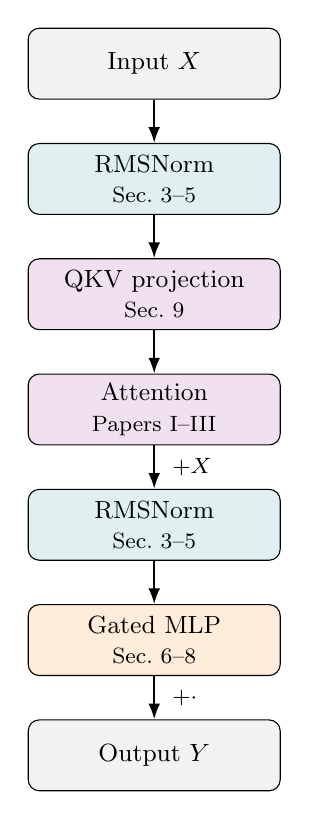
\begin{tikzpicture}[
  node distance=0.55cm,
  box/.style={draw, rounded corners, minimum width=3.2cm, minimum height=0.9cm, align=center, font=\small},
  norm/.style={box, fill=teal!12},
  attn/.style={box, fill=violet!12},
  ffn/.style={box, fill=orange!15},
  io/.style={box, fill=black!5},
  arrow/.style={-{Latex[length=2mm]}, thick}
]
\node[io] (input) {Input $X$};
\node[norm, below=of input] (norm1) {RMSNorm\\\footnotesize Sec.~3--5};
\node[attn, below=of norm1] (proj) {QKV projection\\\footnotesize Sec.~9};
\node[attn, below=of proj] (attn) {Attention\\\footnotesize Papers I--III};
\node[norm, below=of attn] (norm2) {RMSNorm\\\footnotesize Sec.~3--5};
\node[ffn, below=of norm2] (ffn) {Gated MLP\\\footnotesize Sec.~6--8};
\node[io, below=of ffn] (output) {Output $Y$};

\draw[arrow] (input) -- (norm1);
\draw[arrow] (norm1) -- (proj);
\draw[arrow] (proj) -- (attn);
\draw[arrow] (attn) -- (norm2) node[midway, right=0.1cm, font=\footnotesize] {$+X$};
\draw[arrow] (norm2) -- (ffn);
\draw[arrow] (ffn) -- (output) node[midway, right=0.1cm, font=\footnotesize] {$+\cdot$};
\end{tikzpicture}
\caption{The pre-norm transformer block pipeline. Teal: RMSNorm
(this paper, Sections~3--5). Purple: QKV projection (new, Section~9)
and attention (Papers~I--III). Orange: gated MLP (this paper,
Sections~6--8). Residual connections are noted on their respective
arrows.}
\label{fig:block}
\end{figure}

Because each
sublayer's fused cost was derived under the same accounting convention
(full-size activation reads/writes only, with intermediates eliminated
by recomputation wherever MoA's outer-product compatibility permits
it), the block-level fused forward+backward cost is additive. One
addition is needed beyond Papers I--III: those papers treat $Q,K,V$ as
already-given inputs to attention, but a full block must first produce
them from the normalized input $Z_1$ via learned projections $Q =
Z_1\times W_Q$, $K = Z_1\times W_K$, $V = Z_1\times W_V$. This
projection contributes its own memory-optimal cost: forward writes
$Q,K,V$ ($3nd$), and backward writes $G_{Z_1}$ from $G_Q,G_K,G_V$
($nd$), giving
\[
M^{\mathrm{proj}}_{\text{fwd+bwd}} = 4nd,
\]
with $G_Q,G_K,G_V$ themselves counted under attention's own
$M_{\text{fwd+bwd}}$ from Paper II, not double-counted here. As with
every other GEMM in this paper, $W_Q^{\top},W_K^{\top},W_V^{\top}$ and
$Z_1^{\top}$ are reordered-index reads under $\psii$, never
materialized transposes --- the Section~8 lemma extends to the
projection weights without modification. The complete block cost is
therefore
\[
M^{\mathrm{block}}_{\text{fwd+bwd}} =
\underbrace{2 \times 4nd}_{\text{two norms}} +
\underbrace{4nd}_{\text{QKV projection}} +
\underbrace{(4nd_k + 4nd_v)}_{\text{attention (Paper II)}} +
\underbrace{(2nd + 4nd_{\mathrm{ff}})}_{\text{FFN}} +
\underbrace{2nd}_{\text{two residual adds}},
\]
which, taking $d_k = d_v = d$ for a single-head block, simplifies to
$M^{\mathrm{block}}_{\text{fwd+bwd}} = 24nd + 4nd_{\mathrm{ff}}$.
Multi-head decomposition of the projection and attention terms is a
straightforward generalization not elaborated here.

This is, to our knowledge, the first memory-optimal cost function
covering a complete transformer block derived from a single formal
array-algebra framework rather than assembled from separately-optimized
kernels; it gives a direct, apples-to-apples basis for comparing against
measured HBM traffic on GPU hardware (Section 10) and for the
cross-architecture portability arguments (Frontier/Aurora/El Capitan)
made in our DOE-facing framing of the broader MoA program.

\section{Verification and Benchmarking Plan}

\paragraph{Completed.} C/OpenMP and Fortran~90/OpenMP reference
implementations of the RMSNorm forward, backward, and gated MLP
forward, backward DNFs (Sections 3--7) have been verified against a
PyTorch double-precision autograd reference on the grid $B{=}2$,
$N{=}4$, $D{=}8$, $D_{\mathrm{ff}}{=}16$ --- the same $B,N,D$ grid used
for attention verification in Paper II, with $D_{\mathrm{ff}}$ fixed as
the one new dimension the FFN introduces. Both languages parallelize
the per-token forward and backward computation with
\texttt{!\$omp}/\texttt{\#pragma omp parallel for}, and the two
gradient-reduction loops that accumulate across tokens
($G_{\gamma}$ for RMSNorm; $G_{W_{\mathrm{gate}}}$, $G_{W_{\mathrm{up}}}$,
$G_{W_{\mathrm{down}}}$ for the gated MLP) use explicit OpenMP array
reductions rather than a serial post-pass, so the parallel and serial
code paths are the same code, not a fallback. All eight tensors
matched the PyTorch reference to machine precision in both languages at
every thread count tested (1, 2, 4, 8), confirming the reductions are
race-free:

\begin{center}
\begin{tabular}{lcc}
\hline
Tensor & Max abs.\ error, C & Max abs.\ error, Fortran~90 \\
\hline
$Z$ (RMSNorm forward) & $4.4\times10^{-16}$ & $4.4\times10^{-16}$ \\
$G_X$ (RMSNorm backward) & $1.1\times10^{-16}$ & $1.1\times10^{-16}$ \\
$G_{\gamma}$ (RMSNorm backward) & $8.3\times10^{-17}$ & $5.6\times10^{-17}$ \\
$F$ (gated MLP forward) & $1.1\times10^{-16}$ & $1.1\times10^{-16}$ \\
$G_X$ (gated MLP backward) & $2.8\times10^{-17}$ & $4.2\times10^{-17}$ \\
$G_{W_{\mathrm{gate}}}$ (gated MLP backward) & $4.2\times10^{-17}$ & $4.2\times10^{-17}$ \\
$G_{W_{\mathrm{up}}}$ (gated MLP backward) & $5.6\times10^{-17}$ & $5.6\times10^{-17}$ \\
$G_{W_{\mathrm{down}}}$ (gated MLP backward) & $2.8\times10^{-17}$ & $2.8\times10^{-17}$ \\
\hline
\end{tabular}
\end{center}

\emph{Caveat:} the environment used to produce this draft exposed a
single CPU core, so these runs confirm the OpenMP reductions are
race-free at 1, 2, 4, and 8 threads but do not demonstrate real
parallel speedup; a multi-core run to measure actual scaling is listed
as remaining work below, alongside the GPU benchmark.

A fused C/OpenACC kernel implementing the chained pipeline
RMSNorm~$\to$~gated~MLP~forward~$\to$~gated~MLP~backward~$\to$~RMSNorm~backward
in a single \texttt{acc data} region (this section's target) has also been
written and verified against a chained PyTorch reference on the same
grid: the forward outputs $Z$ and $F$ matched to $4.4\times10^{-16}$ and
$1.3\times10^{-15}$ respectively. \emph{Caveat:} this kernel was compiled
and run via GCC's OpenACC host-fallback path, since no CUDA-capable GPU
or \texttt{nvc}/\texttt{pgcc} toolchain was available in the environment
used to produce this draft; every \texttt{\#pragma acc} directive is
standard OpenACC and should offload to an actual GPU unmodified, but the
run performed here is a correctness check only, not a GPU bandwidth or
latency benchmark. That benchmark remains future work, listed below.

In all three implementations, no transpose of $X$, $H$,
$W_{\mathrm{gate}}$, $W_{\mathrm{up}}$, or $W_{\mathrm{down}}$ is ever
materialized: every transposed access in Sections 4 and 6--7 is realized
as a reordered-index read from the original array, exactly as the
transpose-elimination lemma of Section 8 claims, and the numerical
agreement above confirms the reordering is faithful to the DNF in both
CPU languages and under OpenACC's execution model.

Figure~\ref{fig:scaling} shows single-thread wall-clock time versus
sequence length $n$ for both kernels in both languages, on the sweep
$n\in\{32,64,\dots,8192\}$ with $B{=}2$, $D{=}64$,
$D_{\mathrm{ff}}{=}256$. C and Fortran~90 track each other closely at
every size, as expected since both implement the identical DNF; this is
a single-core, single-thread measurement (the environment used to
produce this draft exposed one CPU core), so it demonstrates that the
two language implementations agree in wall-clock behavior, not parallel
speedup, which remains future work per below.

\begin{figure}[h]
\centering
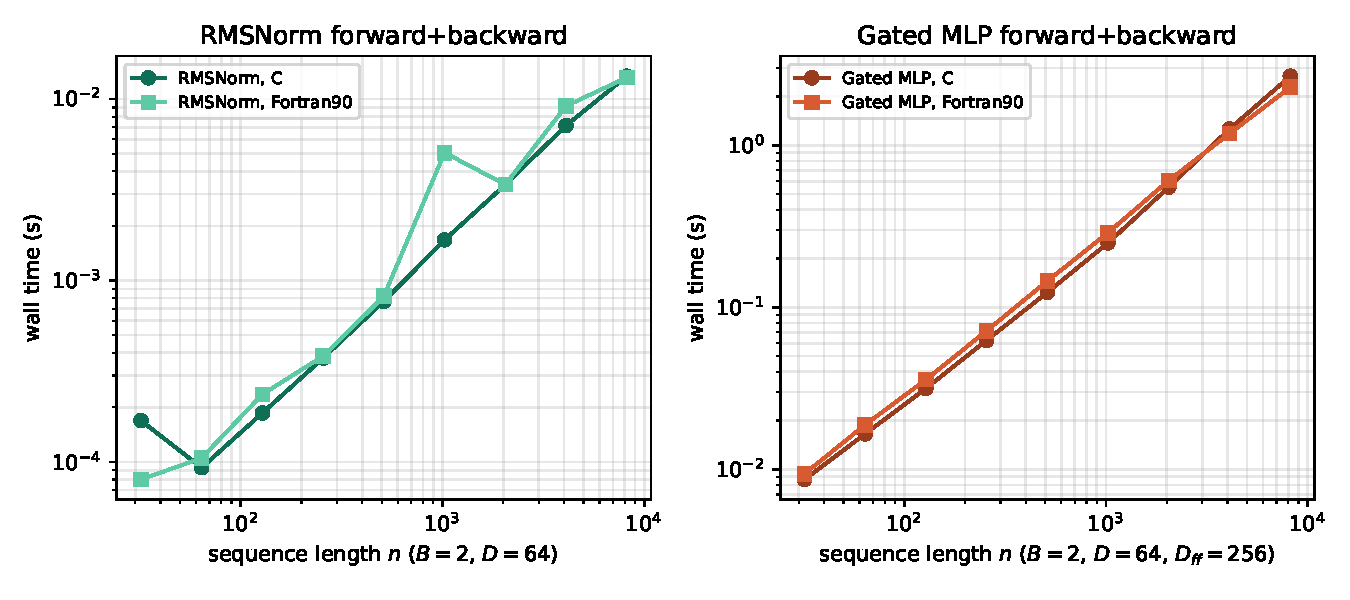
\includegraphics[width=\textwidth]{scaling_plot.pdf}
\caption{Wall-clock time versus sequence length $n$ (log-log), single
thread, $B{=}2$. Left: RMSNorm forward+backward, $D{=}64$. Right: gated
MLP forward+backward, $D{=}64$, $D_{\mathrm{ff}}{=}256$. C and
Fortran~90 implementations track closely, as expected from identical
DNFs. Raw data in \texttt{benchmarking/results\_cpu.csv}.}
\label{fig:scaling}
\end{figure}

\paragraph{Full-block integration (completed).} The item listed as
future work in the previous draft --- extending the fused kernel to
include attention, completing the full pre-norm block in one kernel
--- has been carried out. A C implementation
(\texttt{full\_block\_verify.c}) computes the entire pipeline of
Figure~\ref{fig:block} --- RMSNorm, QKV projection, attention (using the
existing Papers~I--III DNF, adapted inline since that codebase's
functions are compiled against fixed macros rather than exposed as a
callable library), the residual add, RMSNorm again, the gated MLP, and
the second residual add --- forward and backward, against a chained
PyTorch double-precision autograd reference
(\texttt{reference\_full\_block.py}) on the same $B{=}2,N{=}4,D{=}8,
D_{\mathrm{ff}}{=}16$ grid. All ten tensors (the forward output $Y$ and
nine backward gradients: $G_X$, both $G_{\gamma}$, all three QKV
projection weight gradients, and all three FFN weight gradients)
matched to machine precision, $2.8\times10^{-17}$ to
$6.7\times10^{-16}$. A second, independent implementation
(\texttt{full\_block\_gpu\_kernel.c}) performs the identical computation
inside a single OpenACC \texttt{acc data} region --- one HBM round trip
per array across the \emph{entire} block, the literal realization of
the additive $M^{\mathrm{block}}$ claim of Section~9 --- and matches the
same PyTorch reference to the same machine-precision tolerance. As
before, this OpenACC run used GCC's host-fallback path rather than a
physical GPU, so it is a correctness result, not a bandwidth
measurement.

\paragraph{Remaining.} Following the established methodology of Papers
I--III:
\begin{enumerate}
  \item A multi-core run of the OpenMP programs above to measure actual
  parallel speedup, rather than the single-core race-freedom check
  reported here.
  \item An actual GPU run of the fused kernels above (NVIDIA or AMD
  target) to obtain real bandwidth and latency numbers, rather than the
  correctness-only host-fallback runs reported here.
  \item Fortran~90 counterparts to \texttt{full\_block\_verify.c} and
  \texttt{full\_block\_gpu\_kernel.c}, matching the dual-language
  pattern used for the norm and MLP kernels alone.
  \item Benchmarking infrastructure reused from the inference paper's
  PyTorch SDPA comparison, extended to measure end-to-end block latency
  and HBM traffic against the $M^{\mathrm{block}}$ prediction above.
\end{enumerate}

\section{Related Work and Positioning}

\paragraph{Attention kernel fusion.} FlashAttention restructures attention
around IO-awareness, avoiding materialization of the $n\times n$ score
matrix \citep{dao2022flashattention}. FlashAttention-2 improves work
partitioning by parallelizing over the sequence dimension in addition
to batch and head \citep{dao2023flashattention2}, and FlashAttention-3
further exploits newer GPU hardware features such as FP8 precision and
asynchronous tensor-core scheduling \citep{shah2024flashattention3}.
This is precisely the territory Papers I--III of this series already
engage with under a formal MoA derivation rather than a hand-tuned
kernel.

\paragraph{Fused normalization.} NVIDIA's Apex library ships
FusedLayerNorm and FusedRMSNorm as hand-written CUDA
kernels~\citep{nvidia2019apex}, typically benchmarked directly against
native PyTorch implementations for forward-plus-backward wall-clock
speed. Triton-based fused normalization kernels compute the reduction
and the elementwise rescale in a single forward loop, while backward
kernels cache the inverse standard deviation and stage gradient
accumulation in two passes specifically to avoid atomic memory
operations on the parameter gradient~\citep{emergentmind2026fused}.
That engineering choice --- cache the reduction statistic rather than
recompute it --- is the practical analogue of the fused-cost tradeoff we
derive formally in Section~5.

\paragraph{Fused MLP and SwiGLU.} Triton fused kernels combine the two
matrix multiplications, bias additions, the nonlinearity, and the output
elementwise product of a gated MLP into a single kernel
launch~\citep{emergentmind2026fused}. Production serving frameworks
differ in how aggressively they fuse: TensorRT-LLM applies coarser
graph-level pattern-matched fusion, while vLLM and SGLang historically
ran PyTorch's default execution path --- cuBLAS GEMM followed by a
separate SwiGLU kernel --- as the baseline that newer fused kernels are
benchmarked against~\citep{tile2026activation}. The most aggressive
recent work fuses the entire GEMM--activation--GEMM sequence used in
typical multi-kernel SwiGLU implementations into a single deeply fused
operator, reporting single-digit-percent latency gains over the prior
state of the art on current GPU generations~\citep{deepfusion2026kernel}.

\paragraph{Positioning.} Every result above is arrived at empirically:
hand-written CUDA or Triton, tuned by profiling and loop-order search,
one kernel at a time, with no stated general principle for which
intermediate array can be safely eliminated and why. This paper instead
derives elimination as a consequence of MoA's outer-product
compatibility conditions (Sections~3--7) and produces closed-form cost
functions --- $M^{\mathrm{norm}}_{\text{fwd+bwd}}$,
$M^{\mathrm{ffn}}_{\text{fwd+bwd}}$, and the additive
$M^{\mathrm{block}}_{\text{fwd+bwd}}$ of Section~9 --- that predict the
memory-optimal result rather than measure it after the fact. The
transpose-elimination lemma of Section~8 in particular is a single
algebraic statement covering attention, normalization, and the
feed-forward network at once, rather than a separate hand-tuned kernel
per operator family.

\section{Conclusion and Future Work}

Combined with Papers I--III, this paper completes a memory-optimal,
MoA-derived account of a full pre-norm transformer block. Two natural
sequels remain outside this paper's scope by design: a fourth paper
extending the inference-paper's decode DNF and KV-cache artifacts to
dynamic cache management (eviction, paging) and speculative decoding;
and a longer-term research thread testing whether the $\psii$/$\iotaop$/$\gammaop$
primitives extend to the irregular, data-dependent dispatch required for
Mixture-of-Experts routing.

\bibliographystyle{plainnat}
\bibliography{moa_block_theoretical_minimum_v1}

\end{document}
